%************************************************
\chapter{Networking II}\label{ch:networking2}
%************************************************

\section{\mycommand{ping}}

Ping is an utility widely used to check connectivity. It can be used to let a user know if a given internet address can be reached. In case the address is reachable,  I.e., the local machine and the addresses machine, ping also gives the user a ballpark figure for how fast the connection is.

 Ping works by sending an ICMP ECHO\_REQUEST to a destination address provided as an argument, collecting the response from this address, and calculating the time it took for the ICMP packages to be sent back and forth. It can be used as shown below:
\begin{command_line}[make]
ping www.google.com
\end{command_line}


By default, ping keeps sending ICMP requests to the provided address. To stop ping, the user needs to press crtl+C. After finished, ping presents the user with statistics about the transmitted packets, as shown in Listing XXX.

Ping can be used with a number of options to change the number of packets that are sent, the size of such packets, the interval between packets, etc. See Table XXX.

The ping utility is quite useful to check if a connection exists between the local machine and an Internet address. However, in case a connection could not be established, it does not provide any indication on where the problem is. For this goal, another tool called traceroute is used.


\section{\mycommand{traceroute}}

The internet is formed by a plethora of different devices connected together by routers, switches, and hubs. More often than not, two devices are connected not directly, but indirectly by means of multiple hops.

As an example, you can see that the terminals A and B in Figure X are connected via a hub and a router. So, any packet travelling from A to B will 

\begin{figure}[!htbp]
  \centering
        % \documentclass{article}
% \usepackage{tikz}
% \usepackage[active,tightpage]{preview}
%\PreviewEnvironment{tikzpicture}
%\setlength\PreviewBorder{7pt}
\definecolor{lavander}{cmyk}{0.2,0.2,0.2,0}
\definecolor{violet}{cmyk}{0.7,0.70,0.7,0}
\definecolor{burntorange}{cmyk}{0.4,0.4,0.4,0}

\def\lav{lavander!90}
\def\oran{orange!30}

\tikzstyle{peers}=[draw,circle,violet,bottom color=lavander,
                  top color= white, text=violet,minimum width=10pt]
\tikzstyle{superpeers}=[draw,circle,burntorange, left color=burntorange,
                       text=violet,minimum width=20pt]
\tikzstyle{legendsp}=[rectangle, draw, burntorange, rounded corners,
                     thin,bottom color=burntorange, top color=white,
                     text=violet, minimum width=2.5cm]
\tikzstyle{legendp}=[rectangle, draw, violet, rounded corners, thin,
                     bottom color=lavander, top color= white,
                     text= violet, minimum width= 2.5cm]
\tikzstyle{legend_general}=[rectangle, rounded corners, thin,
                           burntor\lavange, fill= white, draw, text=violet,
                           minimum width=2.5cm, minimum height=0.8cm]

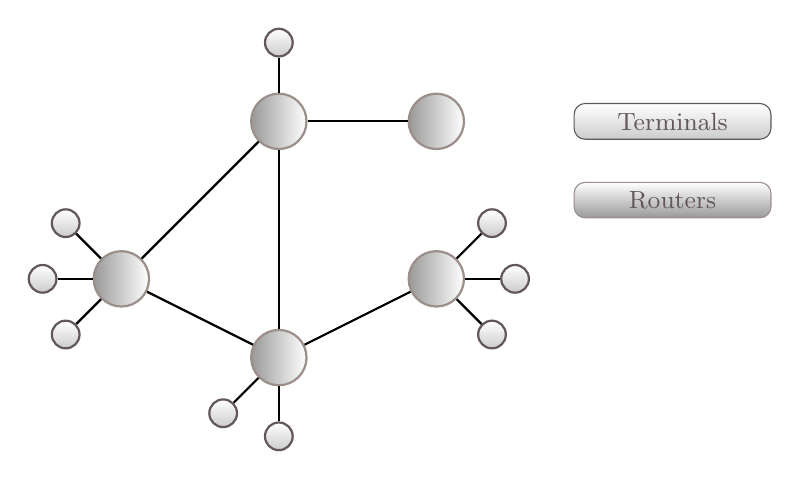
\begin{tikzpicture}[auto, thick]
  % Place super peers and connect them
  \foreach \place/\name in {{(0,-1)/a}, {(2,0)/b}, {(2,2)/c}, {(0,2)/d},
           {(-2,0)/e}}
    \node[superpeers] (\name) at \place {};
  \foreach \source/\dest in {a/b, a/d, c/d,a/e,d/e}
    \path (\source) edge (\dest);
   %
   % Place normal peers
  \foreach \pos/\i in {above left of/1, left of/2, below left of/3}
    \node[peers, \pos = e] (e\i) {};
   \foreach \speer/\peer in {e/e1,e/e2,e/e3}
    \path (\speer) edge (\peer);
   %
   \foreach \pos/\i in {above right of/1, right of/2, below right of/3}
    \node[peers, \pos =b ] (b\i) {};
   \foreach \speer/\peer in {b/b1,b/b2,b/b3}
   \path (\speer) edge (\peer);
   %
   \node[peers, above of=d] (d1){};
   \path (d) edge (d1);
   %
   \foreach \pos/\i in {below left of/1, below of/2}
   \node[peers, \pos =a ] (a\i) {};
   \foreach \speer/\peer in {a/a1,a/a2}
   \path (\speer) edge (\peer);
   %%%%%%%%
   % Legends
   \node[legendsp] at (5,1) {\small{Routers}};
   \node[legendp] at (5,2) {\small{Terminals}};
\end{tikzpicture}

        \caption{Network topology showcasing the connection between terminals T1 and T2.}
        \label{fig:trqceroute}
\end{figure}

\begin{command_line}[make]
traceroute www.google.com
\end{command_line}
